
\chapter[Referencial Teórico]{Referencial Teórico}
Este capítulo apresenta os conceitos teóricos que abordam este trabalho, detalhando a estrutura cerebral responsável pela geração dos sinais de interesse na subseção 2.1, o sistema de captura dos sinais (a EEG) na subseção 2.2, o sistema que se refere às BCIs que realizam a tradução dos sinais em comandos para dispositivos na subseção 2.3, os detalhes técnicos a respeito dos sinais oferecidos pela base de dados \textit{BCI Competition} na subseção 2.4, a estrutura geral de um classificador LDA na subseção 2.5, os conceitos de um SoC na subseção 2.6 e por fim o estado da arte das implementações de algoritmos de classificação na subseção 2.7. 

\section{O Cérebro}
O Sistema Nervoso Central (SNC) é o responsável direto pelo comando do nosso comportamento geral\cite{David_Clarck}. Ele pode ser dividido em três principais áreas: tronco encefálico ou medula espinhal, o cérebro e o cerebelo (Figura \ref{BrainParts}) \cite{alvarezneurobiomecanismos}.

\begin{figure}[h]
	\centering
	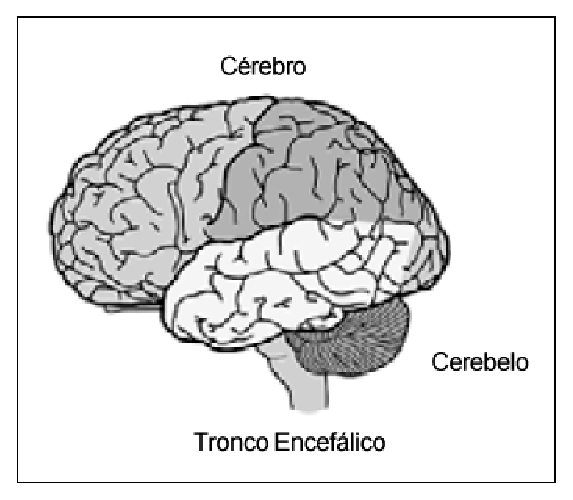
\includegraphics[keepaspectratio=true,scale=1.0]{figuras/estrutura_cerebral.eps}
	\caption{Três principais áreas do cérebro. Fonte: \cite{alvarezneurobiomecanismos}}
	\label{BrainParts}
\end{figure}

O tronco encefálico, parte caldal do SNC recebe e processa todos os sinais dos sensores corporais, além de realizar o controle dos membros e do tronco humano \cite{KANDEL}.

O cérebro é o processador do SNC, nele são recebidos e processados os sinais da medula espinhal, além de fornecer todos os sinais de controle para a própria medula, que por sua vez distribui os sinais para os membros e tronco \cite{KANDEL}.

O cerebelo é localizado logo atrás do tronco encefálico que se conectam através de fibras chamadas de pedúnculos \cite{KANDEL}, é a segunda maior estrutura do SNC contendo mais da metade dos neurônios cerebrais, \cite{SIULYDissertacao} é responsável pelo mapeamento em volta do indivíduo, ou seja, sua percepção \cite{alvarezneurobiomecanismos}, além do controle da região motora e a memória de movimentos \cite{SIULYDissertacao,alvarezneurobiomecanismos}

Os sinais de controle e de sensoriamento são sinais elétricos armazenados nos neurônios \cite{KANDEL}. Suas características eletroquímicas permitem que os neurônios armazenem e transmitam sinais elétricos para qualquer outra célula receptora mesmo que a longa distâncias \cite{SIULYDissertacao}. Sua estrutura pode ser dividida em três principais partes: 1) Corpo da celula, 2) axônio e 3) dendrito, conforme apresentado na Figura(\ref{neuronParts}).
\begin{figure}[h]
	\centering
	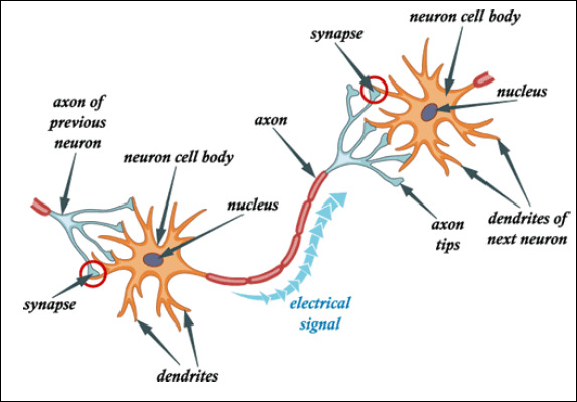
\includegraphics[keepaspectratio=true,scale=1.0]{figuras/Estrutura_neuronio.PNG}
	\caption{Estrutura de um neurônio. Fonte: \cite{SIULYDissertacao}}
	\label{neuronParts}
\end{figure}

A ativação dos neurônios é dada através de um gradiente de concentração eletroquímico, resultando na produção de uma corrente elétrica cerebral que flui através do axônio, o que torna possível a comunicação com outras celulas \cite{SIULYDissertacao}. A corrente elétrica cerebral consiste comumente de íons de Na+, K+, Ca++ e Cl- \cite{EEGSignals}.

As atividades elétricas cerebrais podem ser divididas em dois conjuntos: os potenciais de ação (AP) e os potenciais de sinapse (SP) \cite{SIULYDissertacao}.

Sempre que um potencial de sinapse atinge o limite de condução, ou seja, se o potencial é carregado (estimulado por alguma atividade cerebral) até o ponto em que se é gerada uma corrente elétrica no axônio, um AP é iniciado \cite{SIULYDissertacao}.

Como dito antes, o cerebelo é o responsável pelo controle da percepção e dos movimentos, além da memória de movimento, portanto a percepção, os movimentos e a imagética motora são os estímulos que iniciam uma AP na região do cerebelo \cite{alvarezneurobiomecanismos}.

Os potenciais elétricos gerados a partir dos potenciais de sinapse são armazenados na escalpe (ou couro cabeludo), onde durante uma atividade cerebral é criado um dipolo elétrico entre os dentritos e a soma (região ao redor do núcleo) \cite{SIULYDissertacao}. Estes potenciais podem ser medidos pela eletroencefalografia, conteúdo abordado na seção 2.2 deste trabalho.

\section{Eletroencefalografia}

A Eletroencefalografia (EEG) é um sistema de aquisição de potenciais elétricos, que refletem atividades cerebrais humano \cite{Siulybook}. É muito usado por profissionais de saúde e cientistas para avaliar e estudar funções cerebrais e diagnosticar distúrbios neurológicos \cite{Siulybook}.

A técnica popular que registra sinais do cérebro usando eletrodos estrategicamente colocados sobre o couro cabeludo do paciente, portanto não invasiva, é muito importante nos diagnósticos de doenças neurológicas \cite{raobrain}. Em um exame de EEG , dependendo da sua aplicação, podem ser usados de 1 a 256 eletrodos que iram captar os sinais de forma paralela \cite{raobrain}. Cada par de eletrodos formam um canal, portanto com 256 eletrodos tem-se uma leitura de 128 canais, também conhecido como EEG multi canais \cite{raobrain}. Cada canal recebe um amplificador de instrumentação e um equipamento de gravação do EEG \cite{raobrain}.

Devido às diferentes camadas e tecidos interpostos entre a fonte do sinal (atividade neural no córtex) e os sensores colocados no couro cabeludo, tudo isso atuando como um filtro passa-baixa, faz com o que a resolução 
espacial do EEG seja ruim, em contra partida tem boa resolução temporal na faixa de milisegundos \cite{raobrain}.
 
Em um adulto normal, o sinal típico de EEG tem sua amplitude variando de 1 a 100 microvolt, se for medido usando eletrodos de tipo agulha o seu módulo pode variar de 10 a 20 milivolt. Considera a não uniformidadeb do cérebro humano e a organização funcional do cortex, o sinal de EEG pode variar bastante de acoordo com a disposição dos eletrodos \cite{SIULYDissertacao}.

Com a baixa amplitude desse tipo de sinal, ele pode sofrer facilmente atenuações, contaminações em seu espectro, como por exemplo interferência da rede elétrica de 60 Hz e seus harmônicos associados, e principalmente atividades musculares exercidas no ato da extração dos sinais. Portanto no momento do exame os pacientes são orientados a não realizar nenhum tipo de movimento \cite{raobrain}.

Para especificar um padrão de alocação dos eletrodos na cabeça dos pacientes ou voluntários, é usado o sistema internacional 10-20, esse padrão determina as distancias entre eletrodos \cite{Siulybook}. São posicionados eletrodos primeiramente em pontos estratégicos, os pontos são nomeados por: \textit{mastoids}mastoids, eletrodos de referência localizados atŕas de cada orelha (A1 e A2), \textit{Nasion}, referência no segmento do topo do nariz, porém nivelado com os olhos e por fim, o \textit{onion}, referência situada na base do crânio no ponto médio da parte de trás da cabeça, as medidas são feitas a partir desses pontos, no sentido transversal e médio,  com intervalos de 10 e 20 \% \cite{raobrain}, conforme Figura \ref{padrao1020}.

\begin{figure}[h]
	\centering
	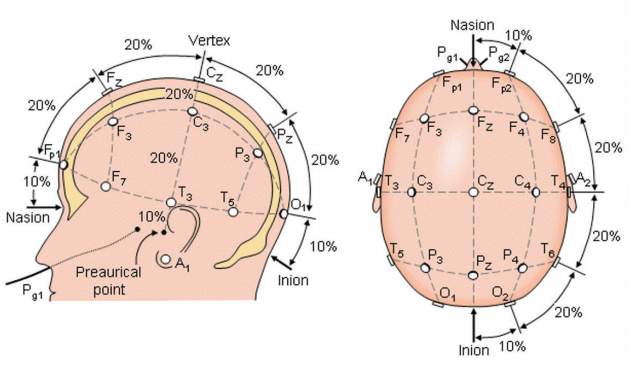
\includegraphics[scale=0.75]{figuras/padrao1020.png}
	\caption{Sistema Internacional de Posicionamento 10-20. Fonte: \cite{campisi2012eeg}.}
	\label{padrao1020}
\end{figure}

A Frequência do sinal é um dos parâmetros mais importantes na avaliação clínica de anomalias em EEGs, e também para compreender o comportamento operacional na pesquisa cognitiva \cite{SIULYDissertacao}.
Com inúmeras oscilações não periódicas milhares de comunicação entre neorônios, comportamentos imprevisíveis o EEG humano é comumente ordenado  em faixas de frequêcias específicas, as bandas são divididas em: delta
 (0.5-4 Hz) , theta($\theta$)(4-8Hz), alpha($\alpha$)(8-13Hz), beta($\beta$)(13-30Hz) e acima de 30Hz gama($\gamma$), conforme Figura \ref{EEGcomun}.
 \newline

\begin{figure}[h]
	\centering
	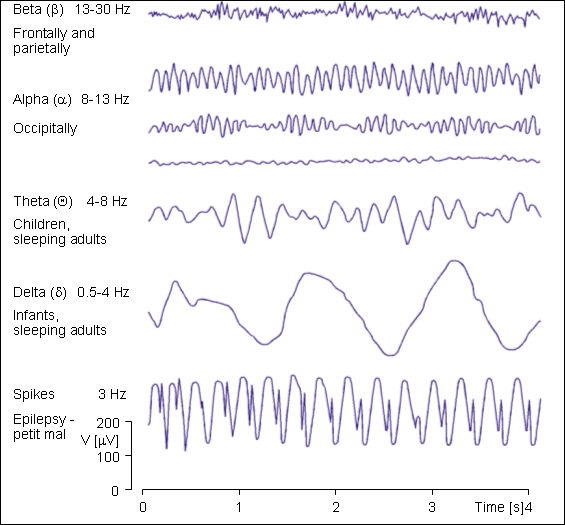
\includegraphics[keepaspectratio=true,scale=0.75]{figuras/formas_EEG.png}
	\caption{Exemplos de diferentes tipos de EEG. Fonte: \cite{campisi2012eeg}}.
	\label{EEGcomun}
\end{figure}

Uma das aplicações dos sinais adquiridos pela EEG são as \textit{Brain Computer Interface} \cite{F.Lotte, SIULYDissertacao}, que é apresentado na seção 2.3.


\section{\textit{Brain Computer Interface}}

Uma \textit{Brain Computer Interface} (BCI) (em português, Interface Cérebro-Máquina) é um sistema que analisa sinais cerebrais e os convertem para um novo sinal de saída \cite{BCIWolpaw}, ou seja, uma BCI é um sistema que realiza a comunicação entre o cerébro e o mundo externo sem a interação neuromuscular \cite{BCIWolpaw}.
O termo BCI foi utilizado pela primeira vez por Jacques Vidal em 1970, onde foram utilizadas técnicas invasivas para aquisição dos sinais cerebrais, sistema de eletrocorticografia (ECoG) \cite{BCIWolpaw}, onde os sensores de aquisição eram instalados na região do cortex. Em 1980 o mesmo Jacques Vidal publicou pela primeira vez a utilização de uma BCI não invasiva utilizando o sistema da EEG \cite{CristophBCI}, as duas técnicas são apresentadas na Figura \ref{ECoGeEEG}.
\pagebreak


\begin{figure}[h]
	\centering
	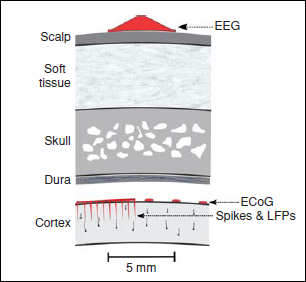
\includegraphics[keepaspectratio=true,scale=1.0]{figuras/sistemas_de_aquisicao.PNG}
	\caption{Diferença entre os sistemas ECoG e EEG. Fonte: \cite{BCIWolpaw}.}
	\label{ECoGeEEG}
\end{figure}

Atualmente é mais comum a utilização do sistema da EEG para aquisição de sinais cerebrais por se tratar de um sistema não invasivo \cite{CristophBCI}. A BCI realiza a tradução dos sinais cerebrais através de seis passos: 1) medição dos sinais cerebrais, 2) pré-processamento destes sinais, 3) extração de características, 4) classificação, 5)tradução dos sinais em comandos e 6) realimentação \cite{MasonAndBirch}, conforme apresentado na Figura \ref{BCI_flow}.

\begin{figure}[h!]
	\centering
	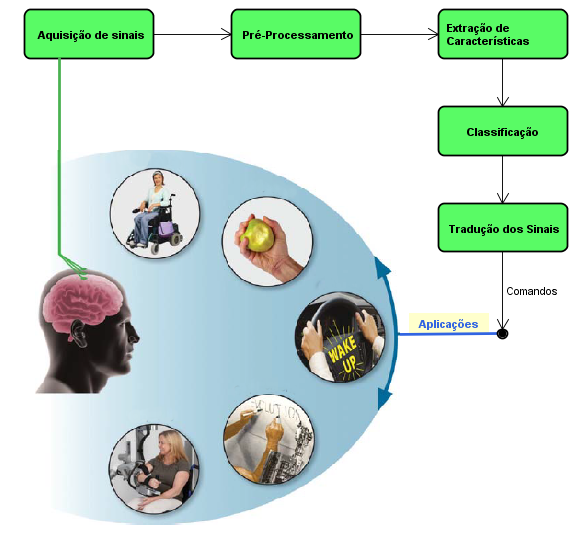
\includegraphics[keepaspectratio=true,scale=0.6]{figuras/Fluxograma_BCI.PNG}
	\caption{Fluxograma de processos de uma BCI, onde pode ser aplicado em mecanismos motorizados, reabilitação muscular, alarmes, entre outros (Adaptado de \cite{BCIWolpaw}).}
	\label{BCI_flow}
\end{figure}

\begin{enumerate}
	\item \textbf{Medição de sinais}: Consiste na primeira etapa de um BCI, onde são medidos potenciais elétricos provenientes de atividades cerebrais \cite{SIULYDissertacao}, os sinais utilizados neste trabalho foram adquiridos utilizando a EEG.
	\item \textbf{Pré-Processamento}: Nesta etapa são utilizados filtros para limpar todo tipo de ruído do sinal e amplificando as informações relevantes dentro do sinal \cite{SIULYDissertacao}.
	\item \textbf{Extração de Características}: Nesta etapa são extraídos dos sinais valores relevantes, chamados de características \cite{SIULYDissertacao}.
	\item \textbf{Classificação}: Nesta etapa as características extraídas no processo anterior são rotuladas em determinadas classes \cite{SIULYDissertacao}. 
	\item \textbf{Tradução em comandos}: Nesta etapa um comando é associado a cada uma das respectivas classes \cite{SIULYDissertacao}.
	\item \textbf{Realimentação}: Por fim é fornecido ao usuário da BCI uma informação a respeito do seu estado mental, qual atividade cerebral foi detectada \cite{SIULYDissertacao}.
\end{enumerate}

Um dos principais passos para a implementação de uma
BCI é a \textbf{classificação}, pois é após este passo que é realizada a tradução dos sinais provenientes da EEG
em comandos de controle \cite{MasonAndBirch}. Para isso são utilizados algoritmos classificadores, onde um tipo de algoritmo de classificação é o LDA, que é detalhado na seção 2.5.

São utilizadas estratégias mentais para definir ao usuário tarefas mentais para gerar características padrões nos sinais cerebrais de acordo com determinada tarefa, para que o classificador possa interpretar corretamente \cite{SIULYDissertacao}. Uma das mais comuns é imagética motora, que caracteriza a imaginação do movimento de um membro do corpo humano \cite{SIULYDissertacao}.  

\section{\textit{BCI Competition}}
A \textit{BCI Competition} é uma competição que promove o desenvolvimento e melhoria da tecnologia voltada para as BCIs, onde são submetidas diferentes técnicas de análise de dados cerebrais \cite{BCICompetition}. Já foram realizadas quatro edições da competição, nos anos de 2001, 2002, 2004 e 2008 \cite{BCICompetition}. Em cada uma destas competições são fornecidos publicamente sinais cerebrais, adquiridos em laboratórios especializados \cite{BCICompetition}. Estes sinais são divididos em dois conjuntos de dados, os dados de treinamento e os dados de teste, que são utilizados para treinamento e teste dos algoritmos dos participantes \cite{BCICompetition}.

\subsection{\textit{BCI Competition III}}
O objetivo do \textit{BCI Competition III} é validar as metodologias de classificação e processamento de sinais cerebrais aplicados em BCIs desenvolvidas pelos participantes da competição \cite{siteBCI}. Esta edição foi realizada entre Maio e Junho de 2004, onde foram disponilizados 8 \textit{datasets} (I, II, II, IIIa, IIIb, IVa, IVb, IVc e V), desenvolvidos com a participação de 49 laboratórios especializados \cite{BCICompetition}.
Para cada um dos \textit{datasets} foram realizadas diferentes tarefas que estimulam atividades cerebrais durante a aquisição dos sinais, configurando assim um objetivo especifico para cada um dos \textit{datasets} \cite{siteBCI}.

\subsection{\textit{BCI Competition III - Dataset IVa}}
O \textit{dataset IVa} refere-se a um conjunto de dados adquiridos através da EEG, onde os sujeitos (indivíduos nos quais foram capturados os sinais) foram submetidos a estimular o cérebro por imagética motora, através de indicações visuais \cite{BCICompetition}. Os indivíduos foram submetidos a realizarem três tarefas, indicadas visualmente por 3.5s cada tarefa, sendo interrompidas em periodos aleatórios entre 1.75s e 2.25s, onde o sujeito era submetido a um periodo de relaxamento \cite{BCICompetition}. As três tarefas de imagéticas motoras foram: (L) mão esquerda, (R) mão direita e (F) pé direito \cite{BCICompetition}.

Foram adquiridos sinais de 5 sujeitos rotulados em \textit{aa, al, av, aw} e \textit{ay}, onde foram executadas no total 280 tarefas por cada sujeito, algumas previamente rotulada (dados de treinamento) em cada instante de tempo onde a tarefa foi executada, outras não rotuladas (dados de teste) \cite{siteBCI}. Estes sinais foram adquiridos, tratados e disponibilizados por \textit{Fraunhofer FIRST, Intelligent Data Analysis Group (Head: Klaus-Robert Müller), and Charité University Medicine Berlin, Campus Benjamin Franklin, Department of Neurology, Neurophysics Group} \cite{BCICompetition}. A tabela 1 apresenta a quantidade de tarefas previamente classificadas (nomeados \#tr) e a quantidade de tarefas não classificadas (nomeadas \#te) para cada sujeito.

\begin{table}[h!]
	\centering
	\caption{Número de tarefas rotuladas e não rotuladas por sujeito \cite{BCICompetition}.}
	\label{my-label}
	\begin{tabular}{lll}
		\textbf{Sujeitos} & \textbf{\#tr} & \textbf{\#te} \\
		\textit{aa} & 168 & 112 \\
		\textit{al} & 224 & 56 \\
		\textit{av} & 84 & 196 \\
		\textit{aw} & 56 & 224 \\
		\textit{ay} & 28 & 252
	\end{tabular}
\end{table}
 
\section{\textit{Linear Discriminant Analisys}}
O LDA é um classificador desenvolvido para explorar as informações no reconhecimento de padrões supervisionados,
as informações conhecidas são contidas num vetor de treinamento previamente disponibilizado \cite{izenmanLDA}.
No algoritmo do LDA as informações de maior relevância são descobertas, enquanto que as de menor são 
eliminadas. O critério usado pelo algoritmo é obter as dimensões que possuem as características mais
distintas das classes padrão.(A Expert System for Stomach Cancer Images with
Artificial Neural Network by using HOG Features
and Linear Discriminant Analysis:
HOG LDA ANN )

Para um melhor entendimento, supõe-se a existência de um conjunto de dados $\vec x$, onde $\vec x = (x_1, x_2,...,x_n)^T$
e $T$ indicando transposição, com características multivariadas, e que cada dado
seja conhecido devido ser proveniente de uma das  classes $y$,tal que, são predefinidas com características
semelhantes aos dados. As classes podem ser exemplificadas como sendo: espécies de plantas,
precença ou ausência de uma condição médica específica, diferentes tipos de tumores, tipos de veículos automotores
entre outros. Para separar as classes conhecidas uma das outras, é atribuido um rótulo a cada classe, então os dados são
representados como dados rotulados \cite{izenmanLDA}.


Devido a indispensabilidade de diminuir as dimensões dos dados de um determinado conjunto, o objetivo do LDA
é reduzir a dimensão do espaço de conjunto de dados, resolvendo o inconveniente da sobreposição \cite{SinghLDA}.

O LDA tem a proposta de encontrar uma transformação ótima para maximizar a proporção de acordo com a equação \ref{eq: Proporção}.
com isso encotrando o vetor $W$ que proporciona a melhor descriminação. (A Linear Discriminant Analysis Using
Weighted Local Structure Information)

\begin{equation}
	\label{eq: Proporção}
	J(W) = \frac { W^T S_B W}{W^T S_W W}
\end{equation}

Onde $S_B$ é a matriz de dispersão entre as classes e $ S_W$ a matriz de dispersão dentro das classes. 

$S_B$ é obtido sengundo a esquação \ref{eq: dispersaosb} 
\begin{equation}
	\label{eq: dispersaosb}
	 S_B = \sum_{j=1}^{c} n_j(m_j - \bar m)(m_j -\bar m)^T 
\end{equation}
onde $c$ é o número de classes, e $\bar m$ o vetor média e  $m_j$ é o vetor de média dos dados 
pertinentes à classe $j$ e $x$ é o vetor de treinamento.

\begin{equation}
	\label{eq: media}
	\bar m = \frac{1}{n}\sum_{i=1}^{n} {x_i}
\end{equation}

\begin{equation}
	\label{eq: media2}
	m = \frac{1}{n_j}\sum_{x \in c j}^{} x
\end{equation}
A matriz de dispersão entre classes é definida pela equaçao \ref{eq: dispersaosw},
\begin{equation}
	\label{eq: dispersaosw}
	 S_B = \sum_{j=1}^{c} \sum_{x \in C j}{} (X - m_j)(X - m_j)^T 
\end{equation}
Para $S_W$sendo uma matriz não-singular, a solução da equação 
\ref{eq: Proporção}, pode ser escrita como: 

 \begin{equation}
	\label{eq: final}
	S_W^{-1} S_B W = \lambda W
\end{equation}
 
onde $\lambda$ é o auto-valor correspondente ao auto-vetor $W$.
\section{\textit{System-on-Chip}}

\textit{System-on-Chip} (SoC), implica que todo sistema que contém funcionalidades implementadas em hardware e software se encontra em um único chip de silício,combinando processamento, lógica de alta velocidade, interface, memória entre outros componentes ao invés de uma implementação maior em vários chips físicos diferentes agrupados em uma placa 
de cicuito impresso \cite{zynqBook}.

São vários os argumentos a favor da escolha de um SoC a uma placa de circuito impresso, pode-se citar que a solução é de menor custo, viabiliza transferência de dados mais rápidas e seguras entre vários elementos do sistema, possui maior velocidade geral do sistema, menor consumo de energia entre vários outros elementos que fortalecem a escolha de um SoC em sistemas discretos com componentes equivalentes \cite{zynqBook}.

\subsection{Aquitetura Simplificada de um SoC}

O conjunto da aquitetura pode se dividir em dois sistemas, sistema de
hardware  e sistema de software. 


No \textbf{Sistema de Hardware}
encontram-se todos os periféricos,
memórias e processadores, para conecta-los
existe um barramento de comunicação
responsável por isso.
Já no \textbf{Sistema de Software}, o software é do tipo stack, e funciona sobre o
processador, que também sustenta os aplicativos que geralmente têm um
Sistema Operacional (SO) para gerência, uma camada em um nível mais baixo
faz a interface com o sistema de hardware \cite{zynqBook}.

 Diagrama
\subsection{\textit{Zybo-Board}}
A Zybo é uma plataforma de desenvolvimento(figura\ref{Zybo Board}), que é equipada com o Z-7010
este que é  o menor integrante da familía Xilinx Zynq-7000.
Baseado na arquitetura Xilinx$^{\textregistered}$ \textit{All-Programmable System-on-Chip} (AP SoC)
o Z-7010 possui em seu encapsulamento um processador ARM Cortex-A9 de 
dois núcleos e um Xilinx 7-Series(FPGA), Esse chip combinado com memórias, entradas 
e saídas de áudio e vídeo, USB, Ethernet, slot SD entre outros periféricos e suportes
proporciona um \textit{kit} para desenvolvedores que procuram uma plataforma de baixo custo
sem perder a capacidade de processamento do Zynq AP SoC \cite{DigilentZybo}.  

\begin{figure}[h]
	\centering
	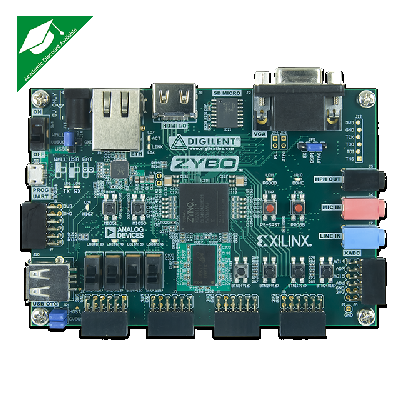
\includegraphics[keepaspectratio=true,scale=1.0]{figuras/zyboboard.eps}
	\caption{Placa de Desenvolvimento Zybo-Board. Fonte: \cite{DigilentZybo}}
	\label{Zybo Board}
\end{figure}



\section{Estado da Arte}
A implementação de algoritmos de classificação em FPGA não é novidade. Em 2003 \cite{RNAFPGA} descreveu um algoritmo de uma rede neural para reconhecimento de faces, obtendo uma acurácia de 92\%. Neste mesmo trabalho realizou a comparação com a implementação em mais duas plataformas \textit{Zero Instrunction Set Computer} e em DSPs, onde obteve melhor resultado na implementação em DSP com acurácia de 98\%.

Os algoritmos de classificação por padrão possuem estrutura bem definida, sobre o \textit{BCI Competition - Data Set IVa}, os melhores resultados obtidos foram de \cite{WangBCIWinner}, onde utilizando do classificador LDA, conseguiu acurácias de 94.17\% geral, 	95.5\% sobre o sujeito (aa), 100.0\% sobre o sujeito (al), 80.6\% sobre o sujeito (av)	100.0\% sobre o sujeito (aw) 97.6\% sobre o sujeito (ay).

A tabela \ref{arte_state} apresenta a acurácia obtida por \cite{F.Lotte} no ano de 2010, no desenvolvimento do algoritmo de classificação LDA, utilizando do algoritmo \textit{Common Spatial Pattern} (CSP) para maximizar a variância do filtro passa-faixa utilizados pelo EEG para uma das classes, enquanto minimiza a variância para as outras demais classes.
\begin{table}[h]
	\centering
	\caption{Acurácia de classificação do algoritmo LDA utilizando do algoritmo CSP para maximização de variância de classes. \cite{F.Lotte}}
	\label{arte_state}
	\begin{tabular}{ll}
		\textbf{Sujeitos} & \textbf{\begin{tabular}[c]{@{}l@{}}Acurácia do LDA com \\ algoritmo CSP\end{tabular}} \\
		\textit{aa} & 66,70\% \\
		\textit{al} & 96,43\% \\
		\textit{av} & 47,45\% \\
		\textit{aw} & 71,88\% \\
		\textit{ay} & 49,60\%
	\end{tabular}
\end{table}
